\documentclass[conference]{IEEEtran}
\usepackage[T1]{fontenc}
\usepackage{amsmath,amssymb}
\usepackage{booktabs}
\usepackage{multirow}
\usepackage{xcolor}
\usepackage{comment}
\usepackage{graphicx}
\graphicspath{{figs/}{./}}
\usepackage[hidelinks]{hyperref}

\begin{document}

\title{SWIFT-HDC: Table-Free Integer Hyperdimensional\\ Learning on a RISC-V SoC}
\begin{comment}


\author{\IEEEauthorblockN{First Author, Second Author}
\IEEEauthorblockA{Department, Institution, City, Country\\
email@institution.edu}}
\end{comment}
\maketitle

\begin{abstract}
Accurate hyperdimensional computing (HDC) needs integer prototypes, iterative retraining and a dot-product search. RISC-V HDC hardware, however, is built for binary prototypes, saturating 0/1 counters and Hamming search, and it stores its level and position hypervectors as tables larger than a microcontroller's entire memory. We present SWIFT-HDC, a PicoRV32-based SoC whose SWIFT core brings integer HDC learning within a microcontroller-class memory budget. Its contributions are (i) table-free encoding: a hash-based generator produces every 32-lane chunk of a level and a position hypervector in the free address cycle of the scratchpad loop, replacing 682\,KB of tables, over 40 times the SoC's main memory, with about 19\,k gates, at no cycle cost, with 18\% less encoding energy than streamed tables and no measurable change in accuracy, whereas a naive hashed generator loses 9 to 19 points; (ii) a fused datapath in which one set of signed weighted MAC lanes performs both encoding and perceptron updates, with a multiplier-free argmax dot search and in-place Q1.15 normalization, so that all learning state stays in one wide scratchpad; and (iii) a one-instruction-per-feature interface over sky130 OpenRAM scratchpads. At equal throughput of 16 elements per cycle, SWIFT needs 4.8$\times$ fewer cycles per clip than the Ara RISC-V vector processor, both measured in cycle-accurate RTL simulation, and an estimated 80$\times$ less energy per clip than the SoC's CPU running the same kernels. A streaming fixed-point front end feeds it video without storing the clip. On KTH action recognition, the bit-exact model of the chip reaches 82.8\% (5 classes) and 70.1\% (6 classes) in leave-one-person-out evaluation, 17 to 24 points above a binary RISC-V HDC unit and 6 to 9 points above an idealized binary design. It reaches 91.9\% on ISOLET, 91.6\% on UCI HAR and 63.9\% on 101-class UCF101 with frozen learned embeddings, where the binary unit reaches 15.3\%. In sky130 the SWIFT core meets 100\,MHz in 8.18\,mm$^2$, of which the complete integer-learning logic, including the generator, is 0.185\,mm$^2$.
\end{abstract}

\begin{IEEEkeywords}
hyperdimensional computing, RISC-V, on-chip learning, video action recognition, hardware accelerator, sky130
\end{IEEEkeywords}

\section{Introduction}
Hyperdimensional computing (HDC) represents data as high-dimensional vectors and classifies by similarity to class prototypes~\cite{kanerva2009}. Its bind, bundle, permute and similarity operations reduce to simple bit-parallel logic. This has produced RISC-V instruction-set extensions and coprocessors~\cite{martino2026,montagna2018}, dedicated engines~\cite{tinyhd,generic} and FPGA accelerators~\cite{li2024eeg,sahruri2026routehd}. Most of these designs store binary prototypes, bundle with saturating 0/1 counters and classify by Hamming distance, and they are evaluated on speech, sensor and biosignal data.

Harder inputs such as video need many feature groups of unequal importance. Accurate HDC classifiers on such inputs need two things a binary pipeline cannot express. The first is a \emph{weighted} accumulation across groups instead of a 0/1 majority counter. The second is \emph{signed} perceptron updates on non-binarized prototypes, followed by a dot-product search. On KTH action recognition, an emulation of a binary RISC-V HDC unit~\cite{martino2026} reaches 53.4\%. The same features with signed, retrained 16-bit prototypes reach 73.6\%. Even an idealized binary design with unbounded counters stops at 64.3\%.

Integer prototypes are known to be more accurate than binary ones, both in software~\cite{onlinehd} and on a dedicated engine~\cite{generic}. What keeps integer HDC learning off microcontroller-class SoCs is memory: the level and position tables of one application take hundreds of kilobytes, integer prototypes are 16 times larger than binary ones, and a straightforward integer datapath needs separate encode, update, normalize and search units with their own buffers. A programmable vector core can run the arithmetic but cannot avoid the table traffic. SWIFT removes the tables by generating hypervectors inside the datapath, lets one set of lanes serve encoding and updates, and keeps every learning step in place in one wide scratchpad.
SWIFT is therefore a memory-centric accelerator by design. In integer HDC learning the arithmetic is additions and sign selections, and the cost is in storing and moving hypervectors. We do not propose a new learning rule; we determine which hardware each step of the known one needs (Table~\ref{tab:decomp}) and organize the datapath around its memory traffic. Table-free encoding is a result of that organization rather than an add-on. The synchronous scratchpads leave the address cycle of every chunk free, and \texttt{BINDGEN} uses that cycle to generate the operands that a conventional design would fetch.

We present SWIFT-HDC (Signed-Weighted hyperdImensional learning For fasT video recognition), an SoC that goes from raw frames to a trained classifier on chip. Its contributions are:
\begin{itemize}
\item \textbf{Table-free encoding in the datapath.} A hash-based generator produces each 32-lane chunk of a level and a position hypervector in the free address cycle of the scratchpad loop. The 682\,KB of level and position tables, their memory and their transfers disappear, at no cycle cost, with 18\% less encoding energy than streaming tables into the datapath, and with no measurable change in accuracy. The construction matters: a naive hashed generator loses 9 to 19 points (Sections~\ref{sec:gen} and~\ref{sec:acc}).
\item \textbf{A fused integer-learning datapath} on sky130 OpenRAM macros. One set of 32 signed weighted MAC lanes serves both encoding and perceptron updates, next to a multiplier-free argmax dot search and in-place L2 normalization into the prototype format (Sections~\ref{sec:nov}--\ref{sec:mem}).
\item \textbf{A one-instruction-per-feature interface.} A PCPI bridge supplies extra operands through CSRs, returns scalar results in registers and memory-maps every scratchpad (Section~\ref{sec:isa}).
\item \textbf{An end-to-end video application.} A streaming fixed-point front end replaces the stored clip with running sums, reducing its storage from 1.7\,Mbit to about 0.23\,Mbit, and feeds the learner (Section~\ref{sec:fe}).
\item \textbf{A rigorous evaluation:} the chip's bit-exact model on three KTH protocols, UCI HAR, ISOLET and UCF101 with paired tests over 20 seed sets, a decomposition of the gain by hardware capability, and RTL-level cycle comparisons with scalar and vector RISC-V cores (Section~\ref{sec:res}).
\end{itemize}

\section{Related Work}
\label{sec:rel}
\emph{RISC-V HDC.} Martino \emph{et al.}~\cite{martino2026} add a configurable HDC unit to RISC-V, with binary bind, bundle (saturating counters), clip, permute, similarity and search instructions on scratchpads; we reimplement it as our baseline. PULP-HD~\cite{montagna2018} runs binary HDC in software on a parallel ultra-low-power cluster. Closest to our system, Li and Fang~\cite{li2024eeg} pair a RISC-V host with an HDC accelerator for EEG; their training is single-pass binary bundling, and they list retraining as future work.

\emph{HDC engines.} Tiny-HD~\cite{tinyhd} is an inference engine with 8-bit class elements trained off chip. GENERIC~\cite{generic} trains and retrains on chip with 16-bit class elements. QuantHD~\cite{quanthd} retrains quantized binary or ternary models. RouteHD~\cite{sahruri2026routehd} studies class-parallel binary search on an FPGA with encoding on the host. OnlineHD~\cite{onlinehd} is a strong floating-point software learner, which we use as a reference. None of these designs generates its hypervectors inside the learning datapath of a CPU-attached unit. For video, HyDRATE~\cite{hydrate2021} targets UCF101 on an FPGA; we found no HDC accelerator that learns video on chip.

\section{Application and Algorithm}
\label{sec:app}
We target KTH action recognition~\cite{schuldt2004}: 25 persons, six actions (boxing, handclapping, handwaving, jogging, running, walking) and 599 clips. Each clip is 64 grayscale frames at $32{\times}32$ (63 frame pairs) and yields 1010 features in six L2-normalized groups: \emph{base} (904: global optical-flow histogram, HOG~\cite{dalal2005} mean, flow-histogram std and HOG std), per-cell $|dx|$ and $|dy|$ mean and std (32 each), two autocorrelation sets of 16 lags on the global flow, and 10 flow percentiles.

Each feature $f$ of group $g$ is quantized to $n_g$ levels (21 for base, 11 otherwise), using a per-feature range taken from the training clips. It is encoded with level hypervectors $L_g$ and position hypervectors $P_{gf}$ in $D=5024$ dimensions (157 chunks of 32 lanes):
\begin{equation}
X=\sum_{g} w_g\sum_{f} L_g[q_{gf}]\odot P_{gf},\qquad y=\mathrm{sign}(X).
\label{eq:enc}
\end{equation}
The base group has weight $w_{\text{base}}=2$ and every other group $w_g=1$, so $|X|\le\sum_g w_g F_g=1914$. Training runs perceptron updates on saturating integer prototypes: on a misclassified clip, $h_{\ell}\mathrel{+}=y$ and $h_{\hat c}\mathrel{-}=y$. It runs for up to 40 epochs, keeps the best validation epoch and then L2-normalizes the prototypes. Inference is $\hat c=\arg\max_k\langle y,h_k\rangle$.

\section{Architecture}
\label{sec:arch}

\subsection{SoC overview}
\label{sec:soc}
Fig.~\ref{fig:soc} shows SWIFT-HDC. A PicoRV32 core~\cite{wolf} (RV32I) issues custom instructions through its Pico Co-Processor Interface (PCPI). A bridge dispatches them to three units: the baseline HDCU, the SWIFT core and a quantizer. The front end produces the 1010 Q16.16 features of a clip, and the firmware passes each one to the quantizer and then to the SWIFT core. The CPU also reaches every scratchpad through memory-mapped windows.

All memories are sky130 OpenRAM macros with one read-write and one read port, in 1, 2, 4 and 8\,KB variants. Main memory is two 8\,KB macros (16\,KB) for code and data. The SWIFT core generates level and position vectors itself (Section~\ref{sec:gen}). Applications that need arbitrary user-supplied vectors use table-based encoding instead. For them, a copy engine streams the vectors from main memory into the bit SPM through the scratchpad's host port, one 32-bit word per cycle.

\begin{figure*}[t]
\centering
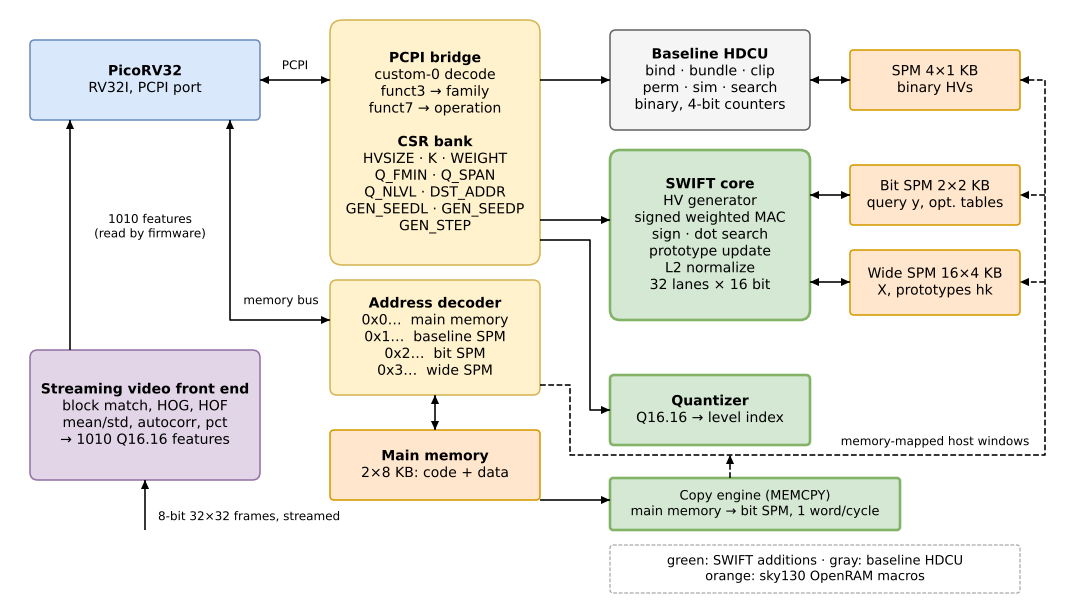
\includegraphics[width=0.86\textwidth]{fig_soc.png}
\caption{SWIFT-HDC SoC. Custom instructions go from PicoRV32 through the PCPI bridge to the baseline HDCU, the SWIFT core or the quantizer. The CPU also reads and writes every scratchpad through memory-mapped windows (dashed). All memories are sky130 OpenRAM macros.}
\label{fig:soc}
\end{figure*}

\subsection{Instruction interface}
\label{sec:isa}
The bridge decodes the RISC-V \texttt{custom-0} opcode: \texttt{funct3} selects the family and \texttt{funct7} the operation (Table~\ref{tab:isa}). PCPI hands a coprocessor the values of \texttt{rs1} and \texttt{rs2} and a writeback path to \texttt{rd}, but never the value held in \texttt{rd}. An operation with a destination and two source scratchpad addresses therefore cannot fit in one R-type instruction.

We follow the CSR approach of the baseline ISA~\cite{martino2026} throughout. Single-cycle CSR instructions write the slow-changing scalars and the destination address, and later operations use them implicitly. These are HVSIZE, the class count $K$, the signed weight, the quantizer's range and level count, \texttt{DST\_ADDR}, and the generator's two seeds and level step. Scalar results (predicted class, level index, Hamming distance and the baseline's search index) return through \texttt{rd}, so the firmware never reads them back from a scratchpad. Weighted accumulation has two opcodes: one clears the accumulator during its sweep and the other adds to it, so the controller keeps no state between instructions.

The bridge is a five-state dispatcher. It asserts \texttt{pcpi\_wait} in the cycle it sees a \texttt{custom-0} instruction, so PicoRV32's coprocessor timeout never starts, forwards the request, waits for the unit's \texttt{done} and asserts \texttt{pcpi\_ready}. It writes \texttt{rd} only for scalar-producing operations, decoded on \texttt{funct3} and \texttt{funct7} together because \texttt{funct7} codes overlap across families. One instruction is in flight at a time and the CPU stalls on it, so CPU accesses to the scratchpads never overlap a controller.

\begin{table}[t]
\caption{Custom instructions (\texttt{custom-0}); cycles at $D{=}5024$, $K{=}5$}
\label{tab:isa}
\centering\scriptsize
\setlength{\tabcolsep}{3pt}
\begin{tabular}{@{}lllr@{}}
\toprule
\texttt{funct3} & Operation (\texttt{funct7}) & Operands $\rightarrow$ result & Cycles \\
\midrule
000 & baseline: bind, bundle, clip, & SPM addresses, as in~\cite{martino2026} & -- \\
    & perm, sim, search, CSRs & sim, search $\rightarrow$ \texttt{rd} & \\
\midrule
001 & \texttt{BINDGEN} (18 / 19) & $q$, $f$, seeds, \texttt{DST}$=X$, $w$ & 314 \\
    & \texttt{BINDMAC} (16 / 17) & $L$, $P$, \texttt{DST}$=X$, $w$ & 314 \\
    & \texttt{PROTO\_UPDATE} (4) & $y$, \texttt{DST}$=h_k$, $w{=}\pm1$ & 314 \\
    & \texttt{SIGN} (2) & $X$, \texttt{DST}$=y$ & 314 \\
    & \texttt{DOTSEARCH} (3) & $y$, prototype base, $K$ $\rightarrow$ \texttt{rd} & 1,570 \\
    & \texttt{NORMALIZE} (5) & $h_k$, \texttt{DST} & $\approx$170k \\
\midrule
010 & CSR write (0--9) & HVSIZE, $K$, WEIGHT, Q\_FMIN, & 1 \\
    & & Q\_SPAN, Q\_NLVL, DST\_ADDR, & \\
    & & GEN\_SEEDL, GEN\_SEEDP, & \\
    & & GEN\_STEP & \\
\midrule
011 & \texttt{QUANTIZE} & feature (Q16.16) $\rightarrow$ level in \texttt{rd} & serial \\
\midrule
100 & \texttt{MEMCPY} & src, $n$ words $\rightarrow$ bit SPM \texttt{DST} & $n{+}5$ \\
\bottomrule
\end{tabular}
\end{table}

\subsection{Baseline HDCU}
The baseline follows~\cite{martino2026}. It has 32-bit SIMD, four 1\,KB scratchpads, 4-bit bundling counters, a 13-bit popcount accumulator, and six functional units (bind, bundle, clip, permute, similarity and search) under a hardware loop that runs each operation over HVSIZE bits. It processes binary vectors only: bundling adds 0 or 1 per lane, clip thresholds an unsigned count with a random tie-break, and search returns the minimum Hamming distance. We keep it in the SoC as the reference, and to show that both units coexist behind one interface.

\subsection{SWIFT core datapath}
\label{sec:nov}
Fig.~\ref{fig:swift} shows the SWIFT core. It processes one 32-lane chunk per step. As in the baseline, its controller loops over the $\lceil D/32\rceil$ chunks in hardware, so software issues one instruction per feature or per prototype update. The lane width $W$ is a build parameter, 16 in the paper configuration (Section~\ref{sec:lane}).

\begin{figure*}[t]
\centering
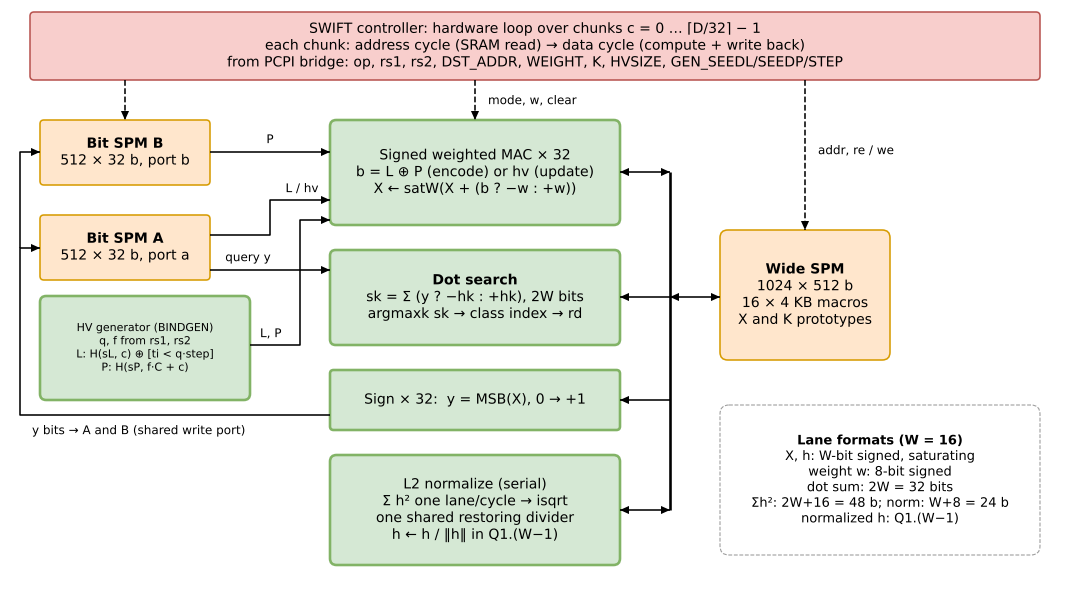
\includegraphics[width=0.86\textwidth]{fig_swift.png}
\caption{SWIFT core datapath. Bit SPMs A and B hold identical copies so that two vectors can be read in one cycle; the sign unit writes both through a shared write port. The wide SPM holds the encode accumulator and the $K$ prototypes; its read-write bus (bold) serves all four units.}
\label{fig:swift}
\end{figure*}

\begin{figure}[t]
\centering
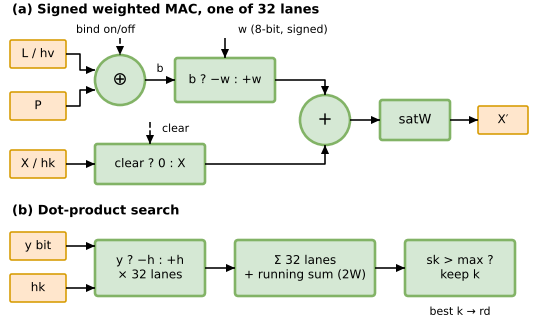
\includegraphics[width=\columnwidth]{fig_lane.png}
\caption{(a) One lane of the signed weighted MAC: the bind can be bypassed for prototype updates, and the accumulator input can be cleared on the first contribution. (b) Dot-product search: per-lane sign selection, a 32-lane adder tree into a $2W$-bit running sum, and a running maximum.}
\label{fig:lane}
\end{figure}

\emph{Signed weighted MAC.} Each of the 32 lanes (Fig.~\ref{fig:lane}a) computes
$X\leftarrow\mathrm{sat}_W\big(X+(b\,?\,{-w}:{+w})\big)$. Here $b=L\oplus P$ is the bipolar product of the level and position bits (bit 1 encodes $-1$) and $w$ is an 8-bit signed weight. This generalizes the baseline's 0/1 counter in two ways: a group's contribution is scaled by $w_g$ before it enters the shared accumulator, and the contribution can be negative. \texttt{PROTO\_UPDATE} reuses the same lanes with the bind disabled ($P{=}0$), so $b$ is the query bit and $w=\pm1$ gives $h_k\mathrel{\pm}=y$. The perceptron update therefore costs no extra datapath. Saturation at $\pm(2^{W-1}{-}1)$ bounds the prototypes without overflow checks in software.

\emph{Sign.} Because $X$ is in two's complement, $\mathrm{sign}(X)$ with ties mapped to $+1$ is the lane's MSB. The binarization needs no comparator array and no random tie-break.

\emph{Dot-product search.} For each prototype, the unit (Fig.~\ref{fig:lane}b) adds $-h_k$ or $+h_k$ per lane into a $2W$-bit running sum, depending on the query bit, and keeps the running maximum and its index. A Hamming search is equivalent ($\langle y,h\rangle=D-2\,\mathrm{Ham}(y,h)$) only once prototypes are binary. During retraining they are wide integers, so the training loop needs this unit. Because the query is binary, the search selects $\pm h$ per lane instead of multiplying 32 pairs of 16-bit values, and needs no multiplier. It returns the class index through \texttt{rd}.

\emph{In-place L2 normalization.} Normalization runs once per prototype after training, so it is built for area rather than speed. The sum of squares is accumulated one lane per cycle in a $(2W{+}16)$-bit register. A sequential integer square root then produces a $(W{+}8)$-bit norm, and one shared restoring divider scales every lane. Serializing the squarer was the largest logic reduction in the core: the 32-lane parallel version was about 85\% of its logic.

No lane can exceed the vector's norm, so every normalized lane lies in $[-1,1)$ and fits a Q1.$(W{-}1)$ word of the same width. Raw and normalized prototypes therefore share the wide-SPM format and normalize in place. A zero-norm prototype is copied unchanged.

\subsection{Table-free hypervector generation}
\label{sec:gen}
Equation~\eqref{eq:enc} needs chunk $c$ of a level vector $L_g[q]$ and of a position vector $P_{gf}$ for every feature. Stored as tables, these vectors take 682\,KB for KTH, more than 40 times the SoC's main memory, and moving two of them into the bit SPM costs two transfers per feature.

\texttt{BINDGEN} instead computes both chunks from two 32-bit seeds per group ($s_L$, $s_P$) while the controller sweeps the chunks. Let $H(s,k)$ be a 32-bit multiply--xorshift hash of $s+k\cdot\phi$, with $\phi$ the golden-ratio constant \texttt{0x9E3779B9}. Lane $i$ of chunk $c$ (dimension $d=32c+i$) is
\begin{align}
L_g[q]_d &= H(s_L,c)_i \oplus \big[\,t_d < q\cdot\Delta_g\,\big], \nonumber\\
t_d &= (d\cdot\phi_{16}+s_L)\bmod 2^{16}, \nonumber\\
P_{gf,d} &= H(s_P,\,fC+c)_i, \nonumber
\end{align}
with $\phi_{16}=\texttt{0x9E37}$, $C=D/32$ and $\Delta_g=2^{16}/(2(n_g{-}1))$.

The level vector of level $q$ flips the lanes whose Weyl-sequence threshold $t_d$ lies below $q\Delta_g$. Consecutive levels therefore differ in $D/(2(n_g{-}1))$ lanes, and the top level differs from the bottom in half of them, the same nested construction as random level tables. In a 21-level group, the similarity of level 0 to levels 1, 10 and 20 is 0.95, 0.50 and 0, exactly as in a random level table.

Each feature reads its own stretch of one hash sequence, so position vectors are independent pseudo-random vectors. At $D{=}5024$, 200 generated position vectors have a mean absolute pairwise correlation of 0.011, the same as 200 random vectors.

The generator is combinational. It has two hash units (one 32-bit add, two xorshifts and one multiplication by a constant each), the index product $fC$, a $q\cdot\Delta_g$ product and 32 16-bit comparators. A generic-gate synthesis estimates it at about 19\,k NAND2 equivalents: that is the logic cost of removing 682\,KB of table storage. Its outputs are registered in the address cycle of each chunk, which the two-phase loop leaves free. \texttt{BINDGEN} therefore keeps the 314-cycle timing of \texttt{BINDMAC} and reads no bit-SPM word.

The firmware writes the seeds and $\Delta_g$ once per group. It then issues one \texttt{BINDGEN} per feature, with the level index from \texttt{QUANTIZE} in \texttt{rs1} and the feature index in \texttt{rs2}. A Python model of the generator is bit-exact with the RTL, and the accuracy model uses it (Section~\ref{sec:acc}).

\subsection{Controller and synchronous memories}
\label{sec:ctrl}
The OpenRAM macros register the read address, so read data appears one cycle after the address. Each chunk loop therefore runs an address cycle, which issues the reads, followed by a data cycle, which computes and writes back. Reads are issued only in address cycles, so no port reads and writes the same word in one cycle, which the macros do not allow.

Every chunk operation costs two cycles. \texttt{BINDGEN}, \texttt{BINDMAC}, \texttt{PROTO\_UPDATE} and \texttt{SIGN} take 314 cycles at $D{=}5024$, and \texttt{DOTSEARCH} takes $2\cdot157\cdot K=1{,}570$. Normalization prefetches each chunk one state ahead of its divide loop and latches it once.


\subsection{Memory organization}
\label{sec:mem}
Fig.~\ref{fig:mem} shows how the firmware allocates both SWIFT scratchpads. On chip there are 24 OpenRAM macros (about 0.7\,Mbit) and no level or position table: as tables, these would take 682\,KB.

\begin{figure}[t]
\centering
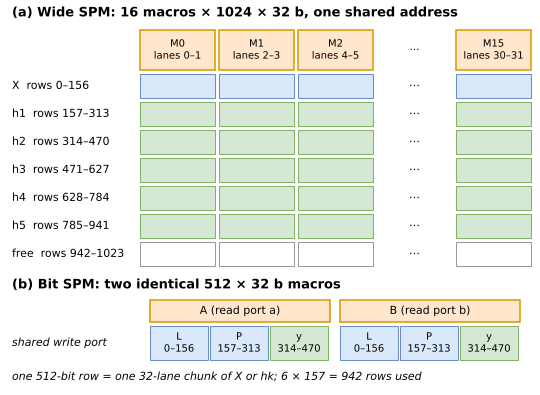
\includegraphics[width=\columnwidth]{fig_mem.png}
\caption{Scratchpad allocation for $D{=}5024$, $K{=}5$. (a) The wide SPM is 16 macros side by side; each holds two 16-bit lanes of every row, so one row is one 32-lane chunk. Prototypes are contiguous, as \texttt{DOTSEARCH} expects. (b) The two bit-SPM copies hold the same data so that $L$ and $P$ can be read together.}
\label{fig:mem}
\end{figure}


\emph{Bit SPM.} With \texttt{BINDGEN} the bit SPM holds only the query $y$. For table-based \texttt{BINDMAC}, the level, position and query vectors take $3\times157$ words (512 allocated, 2\,KB). \texttt{BINDMAC} must read $L$ and $P$ in the same cycle, and each macro has only one read port next to its read-write port. The bit SPM is therefore two identical 2\,KB macros with independent read addresses and a shared write port.

\emph{Wide SPM.} The accumulator and the five prototypes take $6\times157=942$ rows (1024 allocated) of $32W$ bits. With 16-bit lanes a row is 512 bits. It is built from 16 sky130 4\,KB macros (512\,Kbit) that share address and control, each holding one 32-bit slice.

\emph{Host access.} Every scratchpad is memory-mapped (the wide SPM as one sign-extended lane per 32-bit word, with a read-merge-write for lane stores), so the firmware can load hypervectors and inspect prototypes with ordinary loads and stores, which the baseline interface does not allow.

\subsection{Streaming video front end}
\label{sec:fe}
The front end converts raw 8-bit frames into the six feature groups in Q16.16 and reproduces the reference OpenCV/NumPy pipeline exactly: block-matching optical flow over 16 cells ($\pm8$ search, minimum SAD); a motion histogram with octant binning by sign and magnitude comparisons instead of $\arctan$; HOG with OpenCV's reflect-101 gradient, \texttt{fastAtan2} polynomial and L2-Hys normalization; and autocorrelation, percentiles by a sequential sort and per-group L2 normalization.

The clip is never stored. A two-slot frame store with a \texttt{ld\_ready} handshake lets the host overwrite frame $f$ once pair $f$ has been copied into the block-match and HOG units. The per-pair statistics have 484 lanes (HOG, HOF, $|dx|$ and $|dy|$). For each lane, every pair adds $x$ and $x^2$ to running sums, one lane per cycle with one shared multiplier. At the end of the clip,
\begin{equation}
\mu=\frac{S_1}{T},\quad
\sigma^2=\frac{S_2-2\mu S_1+T\mu^2}{T}.
\end{equation}
This is the exact sum of squared deviations from the truncated mean, and it avoids the cancellation of $E[x^2]-E[x]^2$. Only the per-pair global flow ($gdx$, $gdy$) is kept, for autocorrelation and percentiles.

Frame and history storage drops from about 1.7\,Mbit (64 frames plus 63$\times$484 history words) to about 188\,kbit of registers and 40\,kbit of small RAM. HOG gradients are held as 9-bit integers and expanded to Q16.16 at the output, which cuts that buffer from 65 to 18\,kbit.

\subsection{On-chip learning flow}
\label{sec:flow}
Fig.~\ref{fig:flow} shows the firmware loop. The group's seeds and weight are written once per group. For each of the 1010 features, the CPU writes the feature's quantization range, issues \texttt{QUANTIZE} to obtain the level index in a register, and issues \texttt{BINDGEN} with that index and the feature index. After the last feature, \texttt{SIGN} produces the query and \texttt{DOTSEARCH} returns the predicted class. In training, a misclassified clip triggers two \texttt{PROTO\_UPDATE}s, and after the last epoch each prototype is normalized once. Inference is the same loop without updates. All learning state stays in the wide SPM, and the CPU never touches a prototype during training.

\begin{figure}[t]
\centering
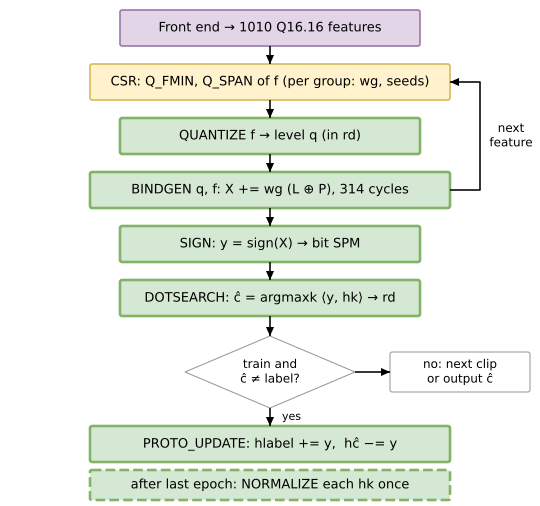
\includegraphics[width=0.92\columnwidth]{fig_flow.png}
\caption{Per-clip firmware flow for on-chip training and inference. Colors follow Fig.~\ref{fig:soc}.}
\label{fig:flow}
\end{figure}

\section{Results}
\label{sec:res}

\subsection{Evaluation setup}
Accuracy comes from a model of the hardware pipeline that is bit-exact with the RTL. It reproduces the Q16.16 front end, the quantizer rounding, integer encoding and saturating training, Q1.$(W{-}1)$ normalization and the integer dot search, so it gives the accuracy of the chip. Mode~E is the chip (16-bit lanes, table-free encoding); E$_{\mathrm{tab}}$ is the same pipeline with random level and position tables. Mode~G emulates the baseline unit: binary bundling limited by 4-bit counters (hierarchical majority in groups of 14), binary prototypes, Hamming search and no retraining, since its ISA has no signed update. Mode~H removes G's counter limit and bounds any binary bundling design of this kind. References are floating-point HDC at the same $D$ and OnlineHD~\cite{onlinehd}.

We use KTH because its low-resolution, fixed-camera clips match what an edge front end can process without a deep network, and because it is the common benchmark for lightweight and spiking video recognition. To test the learner on unconstrained video with learned features, we also run UCF101 (Section~\ref{sec:ucf}).

We use three KTH protocols: the \emph{notebook} split (nine standard test persons, training on the other 16 with a random 15\% validation draw, 5 classes as in the reference model), the \emph{official} split of Sch\"uldt \emph{et al.}~\cite{schuldt2004} (8 training and 8 validation persons, 5 and 6 classes), and \emph{leave-one-person-out} (LOPO, 25 folds).
Main tables average 20 seed sets and sweeps use 10. Each seed set redraws the generator seeds, the random tables of E$_{\mathrm{tab}}$ and of the baseline, the baseline's random tie-breaks and the validation draw. Paired comparisons use the same seed sets, with Wilcoxon signed-rank and paired $t$-tests. Quantization ranges come from training clips only.

\subsection{KTH accuracy}
\label{sec:acc}

\begin{table}[t]
\caption{KTH test accuracy (\%), mean\,$\pm$\,std over 20 seed sets; LOPO pooled over 25 folds}
\label{tab:acc}
\centering\scriptsize
\setlength{\tabcolsep}{2.5pt}
\begin{tabular}{@{}lccccc@{}}
\toprule
& \multicolumn{3}{c}{Fixed split} & \multicolumn{2}{c}{LOPO} \\
\cmidrule(lr){2-4}\cmidrule(l){5-6}
Configuration & 5c notebook & 5c official & 6c official & 5c & 6c \\
\midrule
\textbf{E: SWIFT, 16-bit (chip)} & \textbf{73.6\,$\pm$\,3.4} & \textbf{66.7\,$\pm$\,1.8} & \textbf{56.3\,$\pm$\,2.3} & \textbf{84.0} & \textbf{68.1} \\
E$_{\mathrm{tab}}$: E with random tables & 74.5\,$\pm$\,3.2 & 67.4\,$\pm$\,2.5 & 56.5\,$\pm$\,2.0 & 81.4 & 68.8 \\
E$_{32}$: SWIFT, 32-bit & 73.9\,$\pm$\,2.8 & 66.5\,$\pm$\,1.8 & 56.2\,$\pm$\,2.4 & -- & -- \\
E$_{0}$: SWIFT, no retraining & 66.0\,$\pm$\,2.2 & 62.3\,$\pm$\,1.3 & 52.6\,$\pm$\,1.8 & -- & -- \\
F: binary prototypes, Hamming & 68.6\,$\pm$\,3.4 & 63.1\,$\pm$\,3.0 & 53.5\,$\pm$\,2.7 & -- & -- \\
\midrule
G: baseline HDCU & 53.4\,$\pm$\,3.4 & 47.4\,$\pm$\,3.6 & 39.2\,$\pm$\,3.3 & 59.9 & 50.1 \\
G at $D{=}2048$ (its limit) & 48.8\,$\pm$\,3.2 & 42.3\,$\pm$\,4.3 & 34.9\,$\pm$\,3.6 & -- & -- \\
H: binary, ideal counters & 64.3\,$\pm$\,2.9 & 60.4\,$\pm$\,3.1 & 50.1\,$\pm$\,2.6 & -- & -- \\
\midrule
Float HDC, $D{=}5024$ & 75.6\,$\pm$\,3.1 & 67.9\,$\pm$\,2.4 & 56.3\,$\pm$\,1.8 & 86.4 & 71.3 \\
OnlineHD (float) & 74.5\,$\pm$\,3.0 & 69.1\,$\pm$\,1.9 & 58.7\,$\pm$\,2.3 & -- & -- \\
\bottomrule
\multicolumn{6}{@{}p{0.95\columnwidth}@{}}{\scriptsize --: not evaluated in that protocol. 5c/6c: 5 or 6 classes. LOPO column: one seed set; over five seed sets the chip reaches 82.8\,$\pm$\,1.0 (5c) and 70.1\,$\pm$\,1.6 (6c).}
\end{tabular}
\end{table}

Table~\ref{tab:acc} summarizes KTH. G is the published baseline design as is. H and F are deliberately stronger binary configurations that we construct to test whether a better-provisioned binary unit would suffice. SWIFT beats the baseline accelerator by a wide margin in every protocol:
\begin{itemize}
\item \textbf{Fixed splits:} \textbf{+20.3\,$\pm$\,4.3} points (5-class notebook), \textbf{+19.3\,$\pm$\,3.1} (5-class official) and \textbf{+17.1\,$\pm$\,4.4} (6-class official). SWIFT is better on 20 of 20 seed sets each time ($p_{\mathrm{Wilcoxon}}=8.8\times10^{-5}$).
\item \textbf{Leave-one-person-out:} \textbf{+24.0} points for 5 classes (better for 24 of 25 persons, worse for none, $p=1.7\times10^{-5}$) and \textbf{+18.1} points for 6 classes (25 of 25, $p=1.2\times10^{-5}$).
\item \textbf{Against the baseline at its real 2048-bit bundling limit:} the gap widens to +24.8 points (5-class notebook) and +21.4 (6-class official).
\end{itemize}
Macro-F1 follows accuracy (73.5 vs.\ 52.9 for 5 classes, 55.5 vs.\ 37.6 for 6), so the gain is not concentrated in one class.

\emph{Table-free encoding.} We compare the generated vectors against the same pipeline with random level and position tables (E$_{\mathrm{tab}}$), on the same splits and seed sets. The two are statistically indistinguishable in all eight comparisons: $|\Delta|\le0.8$ points on the three fixed KTH splits ($p\ge0.26$), $+1.3$ and $+0.7$ in LOPO over five seed sets ($p\ge0.11$), and $+0.6$ and $-0.6$ on UCI HAR and ISOLET ($p\ge0.21$).
The 682\,KB of tables can therefore leave the system at no measurable cost. This is by construction: the generated level vectors reproduce the nested flip structure of random level tables exactly, and the generated position vectors are as close to orthogonal as random ones (Section~\ref{sec:gen}).

\emph{Why the generator is built this way.} The level construction cannot be replaced by an arbitrary hash (Table~\ref{tab:gen}). The obvious table-free design generates every level as an independent hash sequence. This destroys the similarity between neighbouring quantization levels and costs 12.3, 14.4 and 11.9 points on the three KTH splits, 9.5 on UCI HAR and 19.3 on ISOLET. It is worse on every seed set ($p_{\mathrm{Wilcoxon}}\le8.8\times10^{-5}$ on KTH) and brings SWIFT down to the level of the idealized binary design H. The nested Weyl-threshold levels are therefore what makes generated encoding work.

Position vectors are less critical: rotations of one hash sequence are statistically equivalent to independent stretches ($|\Delta|\le1.5$ points, $p\ge0.18$). Rotations, however, need two hash evaluations and a 32-bit funnel shifter per chunk, whereas independent stretches need one hash and the index product $fC$, so we use independent stretches.

\begin{table}[t]
\caption{Generator ablation: accuracy (\%) with the chip pipeline, only the hypervectors change}
\label{tab:gen}
\centering\scriptsize
\setlength{\tabcolsep}{2.5pt}
\begin{tabular}{@{}lccccc@{}}
\toprule
Hypervectors & 5c nb. & 5c off. & 6c off. & UCI HAR & ISOLET \\
\midrule
\textbf{Generated (chip)} & \textbf{73.6} & \textbf{66.7} & \textbf{56.3} & \textbf{91.6} & \textbf{91.9} \\
Random tables & 74.5 & 67.4 & 56.5 & 90.9 & 92.4 \\
Independent hashed levels & 61.4 & 52.3 & 44.4 & 82.0 & 72.6 \\
Rotated positions & 75.1 & 67.0 & 56.3 & 91.2 & 92.1 \\
Both shortcuts & 61.3 & 52.5 & 44.6 & 82.1 & 72.1 \\
\bottomrule
\multicolumn{6}{@{}p{0.95\columnwidth}@{}}{\scriptsize KTH: 20 seed sets; UCI HAR, ISOLET: 5 seed sets. Independent hashed levels are worse than the chip on every seed set.}
\end{tabular}
\end{table}

\emph{Where the gain comes from.} Table~\ref{tab:decomp} attributes the gain to the hardware capability that enables it, on the same features and seed sets. Wider bundling counters alone (H) recover 10.9 of the 20.3 points. Signed weighted accumulation with integer prototypes and a dot search, without retraining (E$_0$), adds 1.7 points; retraining through \texttt{PROTO\_UPDATE}, the step prior RISC-V HDC hardware leaves to future work~\cite{li2024eeg}, adds 7.7\,$\pm$\,3.5 (20/20); and keeping the retrained prototypes as integers instead of sign-quantizing them for a Hamming search (F) adds 5.0\,$\pm$\,3.3 (20/20).
The full design leads H by 9.4\,$\pm$\,3.5 points on 20 of 20 seed sets (6.2\,$\pm$\,3.4 for 6 classes, 19/20). A better-provisioned binary unit therefore cannot reach it: those 9 points need the signed datapath, the update path and the integer search together.

\begin{table}[t]
\caption{Accuracy by hardware capability (5-class KTH, 20 seed sets)}
\label{tab:decomp}
\centering\scriptsize
\setlength{\tabcolsep}{3pt}
\begin{tabular}{@{}llc@{}}
\toprule
Configuration & Hardware it needs & Accuracy (\%) \\
\midrule
G: baseline HDCU & 4-bit 0/1 counters, Hamming search & 53.4\,$\pm$\,3.4 \\
H: ideal binary bundling & unbounded 0/1 counters, Hamming & 64.3\,$\pm$\,2.9 \\
E$_0$: SWIFT, single pass & signed weighted MAC, dot search & 66.0\,$\pm$\,2.2 \\
F: retrained, binarized & + \texttt{PROTO\_UPDATE}, Hamming at inference & 68.6\,$\pm$\,3.4 \\
\textbf{E: SWIFT} & \textbf{+ integer dot search, normalize} & \textbf{73.6\,$\pm$\,3.4} \\
Float reference & floating-point datapath & 75.6\,$\pm$\,3.1 \\
\bottomrule
\end{tabular}
\end{table}

\emph{Integer arithmetic.} With the same generated hypervectors and at the same $D$, SWIFT matches floating-point HDC on the 6-class split (56.3\% for both) and stays within 1.2 to 1.9 points of it on the 5-class splits. Neither the lane width nor the fixed-point front end costs accuracy (both under 0.5 points, $p\ge0.32$); the small remaining difference reflects the binarized query that makes \texttt{DOTSEARCH} multiplier-free. Over all runs, the encode accumulator never exceeds 316 in magnitude (bound 1914) and trained prototypes never exceed 82, so saturation never triggers in practice.

\emph{Context.} The original 6-class KTH study, with local space-time features and an SVM, reached 71.7\%~\cite{schuldt2004}. SWIFT reaches 70.1\% in 6-class leave-one-person-out evaluation, from $32{\times}32$ input and with a classifier trained on chip. Nearly all remaining errors fall inside the jogging, running and walking block, the known hard group of KTH; SWIFT's gain over the baseline comes from separating boxing, handclapping and handwaving, which the binary pipeline confuses (handclapping recall 72\% vs.\ 15\%).

\subsection{Standard HDC benchmarks}
To compare with other HDC hardware, we run the same quantizer, encoder and training on UCI HAR~\cite{ucihar} (561 features, 6 classes) and ISOLET~\cite{isolet} (617 features, 26 classes) with their official splits (Table~\ref{tab:uci}). SWIFT reaches 91.6\% and 91.9\%: +31.0 and +54.9 points over the baseline (5/5 seed sets, $p<10^{-6}$), +5.3 and +4.6 over retrained binarized prototypes (5/5, $p\le2.3\times10^{-3}$), and within 1.2 and 1.0 points of floating-point OnlineHD.
On ISOLET it is 12.5 points above the binary RouteHD accelerator (79.4\% at $D{=}10{,}000$, encoding on the host~\cite{sahruri2026routehd}), at half the dimension and while also encoding and training on chip.

\begin{table}[t]
\caption{Standard HDC benchmarks (\%), $D{=}5024$, 5 seed sets}
\label{tab:uci}
\centering\scriptsize
\setlength{\tabcolsep}{4pt}
\begin{tabular}{@{}lcc@{}}
\toprule
Configuration & UCI HAR & ISOLET \\
\midrule
\textbf{SWIFT, 16-bit (chip)} & \textbf{91.6\,$\pm$\,0.4} & \textbf{91.9\,$\pm$\,0.5} \\
SWIFT with random tables (E$_{\mathrm{tab}}$) & 90.9\,$\pm$\,0.9 & 92.4\,$\pm$\,0.4 \\
SWIFT, 32-bit & 90.8\,$\pm$\,0.4 & 92.0\,$\pm$\,0.5 \\
Binary prototypes, Hamming & 86.3\,$\pm$\,1.3 & 87.3\,$\pm$\,0.4 \\
Baseline HDCU & 60.6\,$\pm$\,1.5 & 37.0\,$\pm$\,2.2 \\
OnlineHD (float, software) & 92.8\,$\pm$\,0.3 & 92.9\,$\pm$\,0.2 \\
RouteHD~\cite{sahruri2026routehd} (binary, $D{=}10$k) & -- & 79.4 \\
\bottomrule
\end{tabular}
\end{table}

\subsection{UCF101 with learned embeddings}
\label{sec:ucf}
The SWIFT learner does not depend on hand-crafted features. On UCF101~\cite{ucf101} (13,320 YouTube clips, 101 actions, official split 1), we replace the front end with a frozen ImageNet ResNet-18~\cite{resnet}, the kind of embedding a small vision accelerator or the camera's ISP would provide. Each clip uses 16 frames, and the mean and standard deviation of the 512-dimensional frame embeddings form two feature groups with 64 levels each. Table-free encoding and on-chip retraining run exactly as on KTH (Table~\ref{tab:ucf}). The CNN is never trained: all learning happens in the SWIFT core.

At $D{=}5024$ SWIFT reaches 63.9\%, more than four times the baseline unit's 15.3\%. It retains 91\% of the accuracy of floating-point OnlineHD on the same encoding (70.0\%), whereas the binary unit retains 22\%. The binary pipeline collapses with 101 classes because majority-bundled binary prototypes of many similar classes become nearly indistinguishable under Hamming distance, whereas integer prototypes keep their margins. The lead holds at every dimension: 50.4\% against 4.9\% at $D{=}1024$, and 32.1\% against 2.3\% at $D{=}320$, where all 101 prototypes fit in the existing wide SPM.

\begin{table}[t]
\caption{UCF101 split 1, frozen ResNet-18 embeddings (\%), 3 seed sets}
\label{tab:ucf}
\centering\scriptsize
\setlength{\tabcolsep}{3pt}
\begin{tabular}{@{}lccc@{}}
\toprule
Configuration & $D{=}5024$ & $D{=}1024$ & $D{=}320$ \\
\midrule
\textbf{SWIFT, 16-bit (chip)} & \textbf{63.9\,$\pm$\,1.1} & \textbf{50.4\,$\pm$\,0.0} & \textbf{32.1\,$\pm$\,0.7} \\
Baseline HDCU & 15.3\,$\pm$\,0.4 & 4.9\,$\pm$\,0.8 & 2.3\,$\pm$\,0.3 \\
OnlineHD (float) & 70.0\,$\pm$\,0.4 & -- & -- \\
Wide-SPM rows ($K{=}101$) & 16,014 & 3,264 & 1,020 \\
\bottomrule
\end{tabular}
\end{table}

\subsection{Efficiency of learning}
Fig.~\ref{fig:sweeps}a shows accuracy against hypervector dimension. SWIFT at $D{=}1024$ (66.9\%) beats the baseline at $D{=}8192$ (56.9\%), and it beats the ideal-counter bound at any dimension (at most 64.4\%). At $D{=}1024$ an inference needs 65\,k core cycles instead of 319\,k at $D{=}5024$, so a designer can trade dimension for latency and memory and still lead the full-dimension baseline by 13 points. The same holds along the other axes. With 16 frames per clip SWIFT reaches 68.2\%, 14.6 points above the baseline with 64 frames; with 20\% of the training clips it reaches 57.6\%, above the baseline trained on all of them (54.8\%). Retraining converges within a few epochs (median best epoch 2), with prototype updates falling from 72 in the first epoch to 0 by the fifteenth. Accuracy stays within 71.6--74.3\% from 5 to 63 levels per feature. The gain is not bought with storage: at $D{=}512$ SWIFT's accumulator and prototypes take 49\,Kbit, about 1.5 times the baseline's 32\,Kbit, and reach 61.2\%, 7.6 points above the baseline at $D{=}5024$.

\begin{figure}[t]
\centering
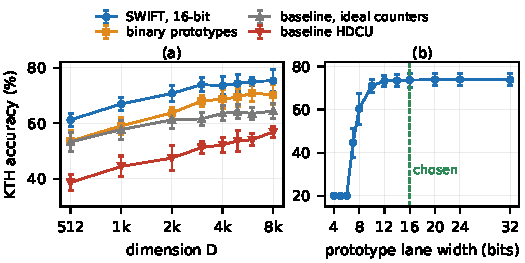
\includegraphics[width=\columnwidth]{fig_res_sweeps}
\caption{5-class KTH accuracy (10 seed sets, mean\,$\pm$\,std) against (a) hypervector dimension and (b) prototype lane width at $D{=}5024$.}
\label{fig:sweeps}
\end{figure}

\subsection{Lane width}
\label{sec:lane}
Fig.~\ref{fig:sweeps}b sweeps the prototype lane width. Accuracy is flat from 12 to 32 bits, and 16-bit lanes equal 32-bit lanes on every benchmark: $-0.2\,\pm\,2.0$ points on 5-class KTH ($p=0.62$), +0.1 on 6-class, +0.8 on UCI HAR and $-0.1$ on ISOLET. Twelve-bit lanes lose 0.4 and 1.1 points (5 and 6 classes) and 8-bit lanes lose 13.2 and 17.0, because Q1.$(W{-}1)$ normalized prototypes become too coarse to rank classes. We therefore build the wide SPM with 16-bit lanes: 16 instead of 32 macros, which saves 7.43\,mm$^2$ of SRAM in sky130 (Table~\ref{tab:area}). GENERIC arrived at the same width for on-chip training~\cite{generic}.

\subsection{Dedicated hardware versus programmable cores}
\label{sec:sw}
To test whether a programmable core could run the same algorithm, we implemented each SWIFT operation in software for two RISC-V cores, at $D{=}5024$, 16-bit saturating lanes and $K{=}5$ (Table~\ref{tab:sw}). On the SoC's own PicoRV32 (RV32I, C, \texttt{clang -O3}), cycles were counted in RTL simulation with a single-wait-state memory. For the vector baseline we use Ara~\cite{ara}, an open-source RVV~1.0 processor with a CVA6 host, and measure every kernel in cycle-accurate Verilator simulation of its RTL, with RVV intrinsics (\texttt{clang -O3}) strip-mined at the full vector length ($e16$, LMUL\,4), results checked against a scalar reference.
With 4 lanes Ara has a 256-bit datapath, 16 16-bit elements per cycle. This is exactly the throughput of SWIFT's 32 lanes at two cycles per chunk; we also report 2 lanes. Ara's testbench memory is an ideal on-chip L2, which favors Ara.

The scalar core spends about 2,200 cycles per chunk on \texttt{BINDMAC}. One clip takes about 350\,M cycles (3.5\,s at 100\,MHz), longer than the 2.56\,s clip itself, so a CPU-only design cannot keep up with the video.

The vector processor does far better but stays well behind SWIFT at equal throughput. On 4-lane Ara, \texttt{BINDMAC} takes 1,935 cycles against SWIFT's 314. Each strip needs two byte loads for the packed tables, an XOR, a load, a merge of $\pm w$ under the mask, a saturating add and a store. This chain of short dependent vector instructions keeps Ara far below its peak throughput. \texttt{DOTSEARCH} is 8$\times$ slower than on SWIFT because each class ends in a reduction. Per clip, 4-lane Ara needs 1.97\,M cycles and 2-lane Ara 3.86\,M.

SWIFT with table-free encoding, measured end to end in the SoC including the CSR writes and instruction issue for every feature, needs 400 cycles per feature and about 0.41\,M cycles per clip: 4.8$\times$ fewer than 4-lane Ara, which reads its tables from ideal memory, 9.4$\times$ fewer than 2-lane Ara, and about 850$\times$ fewer than the scalar core.
On the kernels alone, the gap to 4-lane Ara at equal throughput is 6.2$\times$ (319\,k against 1.97\,M cycles per clip). Table-free encoding also halves SWIFT's own clip time. With stored tables, the vectors must first reach the bit SPM, which costs 770 cycles per feature (0.80\,M per clip) with the copy engine and 13.6\,k per feature with PicoRV32 loads and stores. Generating the vectors in the datapath removes this data movement altogether.

\begin{table}[t]
\caption{Cycles per operation and per clip ($D{=}5024$, $K{=}5$, 16-bit lanes)}
\label{tab:sw}
\centering\scriptsize
\setlength{\tabcolsep}{3pt}
\begin{tabular}{@{}lrrrr@{}}
\toprule
 & RV32I & \multicolumn{2}{c}{Ara (RTL)} & \\
\cmidrule(lr){3-4}
Operation & sw & 2 lanes & 4 lanes & SWIFT \\
\midrule
\texttt{BINDMAC} & 345,155 & 3,794 & 1,935 & 314 \\
\texttt{SIGN} & 116,502 & 2,717 & 1,369 & 314 \\
\texttt{DOTSEARCH} & 766,008 & 23,745 & 12,645 & 1,570 \\
\texttt{PROTO\_UPD.} & 342,789 & 4,002 & 2,027 & 314 \\
\midrule
Per clip, kernels & 349.5\,M & 3.86\,M & 1.97\,M & 319\,k \\
Per clip, end to end & 349.5\,M & 3.86\,M & 1.97\,M & \textbf{0.41\,M} \\
\quad with tables, copy engine & & & & 0.80\,M \\
\bottomrule
\multicolumn{5}{@{}p{0.97\columnwidth}@{}}{\scriptsize All columns measured in cycle-accurate RTL simulation and checked against a scalar reference. Ara uses ideal L2 memory (an upper bound for Ara) and the same bit-packed tables. SWIFT end to end: measured in the SoC with table-free encoding; \texttt{QUANTIZE} is excluded because every option needs it.}\\
\end{tabular}
\end{table}

\subsection{Implementation}
\label{sec:impl}
The baseline HDCU, the SWIFT core and the SoC were synthesized separately with Cadence Genus in SkyWater sky130 (\texttt{sky130\_fd\_sc\_hd}, typical corner, 1.8\,V, 25\,$^\circ$C), with every memory as a sky130 OpenRAM macro (Table~\ref{tab:area}). All three meet the 100\,MHz target with 16-bit lanes.

\begin{table}[t]
\caption{sky130 synthesis results at 100\,MHz}
\label{tab:area}
\centering\scriptsize
\setlength{\tabcolsep}{3pt}
\begin{tabular}{@{}lcccc@{}}
\toprule
Block & SRAM macros & SRAM & Logic & Total \\
 & & (mm$^2$) & (mm$^2$) & (mm$^2$) \\
\midrule
Baseline HDCU & 4$\times$1\,KB & 0.763 & 0.023 & 0.786 \\
\textbf{SWIFT, 16-bit} & 2$\times$2\,KB + 16$\times$4\,KB & 7.995 & \textbf{0.185} & \textbf{8.180} \\
SWIFT, 32-bit & 2$\times$2\,KB + 32$\times$4\,KB & 15.422 & 0.377 & 15.799 \\
SoC, 16-bit & + 4$\times$1\,KB + 2$\times$8\,KB & 10.335 & 0.300 & 10.634 \\
\bottomrule
\end{tabular}
\end{table}

The complete integer-learning logic of the SWIFT core takes 0.185\,mm$^2$ (24\,k cells, 1,577 flip-flops), 2.3\% of the core. It includes the hypervector generator, 32 signed MAC lanes, the dot search and the normalizer. The remaining 97.7\% is the prototype and query storage, which every integer HDC learner needs; SWIFT adds no table storage on top of it. The 16-bit lanes chosen in Section~\ref{sec:lane} halve both the largest memory and the logic: 32-bit lanes would need 15.80\,mm$^2$. In the full SoC, which adds the CPU, the baseline unit and main memory, the HDC learning logic remains a small fraction of the 10.6\,mm$^2$.

\emph{Energy.} We estimate logic power from the synthesized netlists with OpenSTA, annotating flip-flop outputs, SRAM read data and inputs with the toggle rates of the firmware simulation for each operation; on the baseline unit this reproduces Genus's register power within 6\%. The OpenRAM liberty models charge the same power on every clock edge whether or not a macro is accessed, so SRAM energy is computed from the per-macro accesses counted in simulation and the per-access power of the OpenRAM datasheets (within 15\% of the liberty model while every macro is accessed). We use these estimates comparatively:
\begin{itemize}
\item Encoding is 99.6\% of a clip's energy in the core; of each \texttt{BINDGEN}, 72\% is spent in the wide SPM and 28\% in logic.
\item The core's logic draws the same power during \texttt{BINDGEN} as during \texttt{BINDMAC} (within 0.4\%): generating the hypervectors costs no measurable power.
\item Per feature, table-free encoding uses 18\% less energy than table-based encoding with the copy engine and at least 4.2$\times$ less than with CPU copies.
\item 16-bit lanes use 43\% less energy per feature than 32-bit lanes; a training step's two \texttt{PROTO\_UPDATE}s add 0.2\% to a clip's inference energy.
\item The same kernels on PicoRV32 cost at least 80$\times$ more energy per clip, counting only the SoC's clocking and instruction fetches over the 350\,M cycles.
\end{itemize}

\begin{table*}[t]
\caption{Comparison with HDC hardware (reported numbers; nodes and platforms differ)}
\label{tab:cmp}
\centering\scriptsize
\setlength{\tabcolsep}{4pt}
\begin{tabular}{@{}lcccccc@{}}
\toprule
& Tiny-HD~\cite{tinyhd} & GENERIC~\cite{generic} & Li \& Fang~\cite{li2024eeg} & RouteHD~\cite{sahruri2026routehd} & Baseline~\cite{martino2026} & \textbf{This work} \\
\midrule
Platform & 22\,nm ASIC$^\dagger$ & 14\,nm ASIC & FPGA + 16\,nm (sim.) & Alveo U200 FPGA & RISC-V & sky130 + OpenRAM \\
Task (classes) & -- & -- & EEG emotion (2) & ISOLET (26) & -- & KTH (5/6), UCF101 (101), UCI HAR, ISOLET \\
Dimension $D$ & -- & -- & 2000 & 10,000 & configurable & 5024 \\
Prototype elements & 8-bit & 16-bit & binary & binary & binary & 16-bit \\
Encoding on chip & -- & -- & yes & no (host) & yes & yes, table-free \\
Training on chip & no & yes & single pass & no & single pass & yes \\
Iterative retraining & no & yes & no (future work) & no & no & yes \\
CPU integration & -- & -- & RISC-V & -- & RISC-V & RISC-V \\
Video front end & no & no & no & no & no & yes \\
Accuracy (\%) & -- & -- & 79.0 / 86.0 & 79.4 & 53.4 (KTH, ours) & 82.8/70.1 KTH, 63.9 UCF, 91.9 ISOLET \\
Area (mm$^2$), reported & 0.50 & 0.30 & 0.596 & -- & -- & 8.18 (core) \\
Area (mm$^2$), at 130\,nm$^\ddagger$ & 18.9 & 31.1 & 48.0 & -- & -- & 8.18 \\
\bottomrule
\multicolumn{7}{@{}p{0.97\textwidth}@{}}{\footnotesize $^\dagger$ synthesized at 45\,nm and scaled to 22\,nm by its authors. $^\ddagger$ scaled to 130\,nm (sky130) with DeepScaleTool~\cite{deepscale,stillmaker2017}; 16\,nm uses factors interpolated between 14 and 22\,nm. FPGA results are not scaled. Logic-derived factors only approximate SRAM scaling, so scaled values are indicative.}
\end{tabular}
\end{table*}

Table~\ref{tab:cmp} places SWIFT-HDC among HDC hardware. To compare across nodes, we scale reported ASIC areas to 130\,nm with DeepScaleTool~\cite{deepscale}, which applies the fitted device-scaling equations of~\cite{stillmaker2017}; the area factor from 14\,nm to 130\,nm is 104$\times$. At 130\,nm the SWIFT core occupies 8.18\,mm$^2$, against 31.1\,mm$^2$ for GENERIC and 48.0\,mm$^2$ for Li and Fang's accelerator. SWIFT-HDC is the only design that combines on-chip encoding without tables, integer prototypes with iterative retraining, RISC-V integration and a video front end. It is also the only one evaluated on video.

\subsection{Latency}
\label{sec:lat}
Classifying a clip needs about 3.2\,ms of SWIFT-core time at 100\,MHz (317\,k cycles of encoding, 1.6\,k of search), or about 4\,ms end to end in the SoC. The front end processes a frame pair in about 362\,k cycles, so a 64-frame clip takes about 0.23\,s against 2.56\,s of video: the full pipeline runs about 11$\times$ faster than real time. On the PicoRV32 alone the HDC work takes about 350\,M cycles, longer than the clip itself. The accelerator is what turns the learner from the bottleneck into a small fraction of the latency: without SWIFT, HDC learning is 94\% of the clip time; with it, under 2\%. Training repeats this work for every clip in every epoch, so this is the part of the system that on-device learning multiplies. The 16\,KB main memory holds the firmware and the per-group seeds; with \texttt{BINDGEN}, no level or position table exists anywhere in the system.

\section{Discussion}
\label{sec:disc}
\emph{Scaling.} The architecture turns the cost of a learning task into explicit design equations. With $C=\lceil D/32\rceil$ chunks, $F$ features and $K$ classes,
\begin{align}
\text{wide-SPM rows} &= (K{+}1)\,C, \nonumber\\
\text{cycles per clip} &= 2C\,(F + 1 + K), \nonumber\\
\text{cycles per update} &= 4C. \nonumber
\end{align}
The scratchpad bandwidth is fixed by the lane count and does not grow with $K$ or $D$; only capacity and time grow, linearly. Designers can trade dimension for classes within the same memory. All 26 ISOLET classes fit in the existing 512\,Kbit wide SPM at $D{=}1184$ ($27\times37=999$ rows) and reach 87.0\,$\pm$\,0.7\%, 65 points above the baseline at the same dimension (21.5\%, 5/5 seed sets). UCI HAR fits at $D{=}4672$ (1022 rows) at 91.4\,$\pm$\,0.9\%. On KTH, at $D{=}2048$ and with 41\% of the storage, SWIFT (70.7\%) still leads the baseline at full dimension by 17 points (Fig.~\ref{fig:sweeps}a).

Capacity scales with the task while the datapath, its bandwidth and its logic area stay fixed: each additional bank of 16 macros adds 1024 rows, and the equations above size it. Growth linear in $K$ is shared by every prototype or linear classifier. A floating-point linear classifier on the same 1024-dimensional UCF101 embeddings stores $101\times1024$ weights, 1.7\,Mbit even at 16 bits: the same order as SWIFT's 1.7\,Mbit of used rows at $D{=}1024$.

\emph{Generality.} SWIFT implements record-based encoding with retraining and similarity search, the formulation used by the accurate HDC classifiers in software and hardware~\cite{onlinehd,generic}. Its primitives (weighted signed accumulation, generated level and position vectors, signed updates and dot search) are not tied to one application or feature type. The same instructions, firmware and datapath run motion features (KTH), inertial signals (UCI HAR), speech (ISOLET) and CNN embeddings of unconstrained video (UCF101). Only the quantizer ranges, the number of levels and the generator seeds change. Other encodings map onto the same lanes: n-gram encoding is a rotation of the position stream, and random projection is \texttt{BINDMAC} with stored vectors. The front end is the application-specific part of the SoC, and the learner does not depend on it: UCF101 replaces it with a frozen CNN and changes nothing in SWIFT (Section~\ref{sec:ucf}).

\emph{Training cost.} A training step adds at most two \texttt{PROTO\_UPDATE}s (628 cycles) to the 319\,k cycles of inference, under 0.2\% of its time and energy, and retraining converges in about two epochs. On-chip adaptation therefore costs a few passes over a user's clips, with additions and sign selections only, no gradients and no off-chip state.

\section{Conclusion}
SWIFT-HDC shows that integer HDC learning fits a microcontroller-class SoC once its memory problem is solved in hardware. Generating level and position hypervectors in the free address cycle of the scratchpad loop removes 682\,KB of tables at no cycle cost and with no measurable change in accuracy; one set of signed weighted MAC lanes serves encoding and perceptron updates; and a multiplier-free dot search with in-place normalization keeps all learning state in one wide scratchpad.
At equal throughput, the core needs 4.8$\times$ fewer cycles per clip than a RISC-V vector processor, an estimated 80$\times$ less energy than the SoC's CPU, and its complete learning logic takes 0.185\,mm$^2$ in sky130 at 100\,MHz. On KTH, its bit-exact model beats a binary RISC-V HDC unit by 17 to 24 points in every protocol and an idealized binary design by 6 to 9 points. It reaches 91.6 to 91.9\% on UCI HAR and ISOLET, and 63.9\% on 101-class UCF101 with frozen embeddings, where the binary unit reaches 15.3\%. Further generator modes for n-gram and projection encodings, and banked prototype memories for many-class tasks, extend the same datapath.

\bibliographystyle{IEEEtran}
\bibliography{references}

\end{document}
